\chapter{Testautomatisierung mit Selenium}
\label{sec:testautomatisierung_mit_selenium}

Laut Seidel et al. \cite[vgl. S. 48]{seidl_basiswissen_2012} ist der am meisten verbreitete \frqq Angriffspunkt\flqq\ für Testautomatisierung die grafische Benutzerschnittstelle. Seidel et al. \cite[S. 48]{seidl_basiswissen_2012} nennen dafür folgende Gründe:
\begin{itemize}
\item \glqq Sie ist für Tester und Automatisierer anschaulich und leicht greifbar.\grqq
\item \glqq Sie stellt zumeist das Verhalten im realen Umfeld am besten nach.\grqq
\item \glqq Die Dokumentation von Systemen ist auf dieser Ebene meist am vollständigsten.\grqq
\item \glqq Der klassische Systemtest wird oft über diese Schnittstelle abgewickelt.\grqq
\item \glqq Hinter der grafischen Benutzerschnittstelle liegende Systeme werden implizit getestet.\grqq
\end{itemize}
Ein großer Teil der heutzutage entwickelten Anwendungen werden in Form einer Webapplikation realisiert. Im Bereich der Testautomatisierung die als Schnittstelle die grafische Benutzeroberfläche verwenden, stellen diese Webapplikation einen Sonderfall dar.
Im Gegensatz zu gewöhnlichen Denktopanwendungen gibt es bei dieser Art von Anwendung laut Seidel et al. \cite[vgl. S. 88]{seidl_basiswissen_2012} \glqq keinen spezifischen Client für eine Applikation, sondern einen generischen - den Browser.\grqq\ Dies schafft nach Seidel et al.  \cite[vgl. S. 59]{seidl_basiswissen_2012} \glqq für Werkzeuge eine sehr gute Basis, um auf die Elemente der Seite zuzugreigen.\grqq\ Die einzelnen HTML-Elemente und deren Attribute können verwendet werden um die Bestandteile eine Seite zu adressieren.
Ein weit verbreitetes Tool für die Automatisierung, welches diesen Ansatz verfolgt ist Selenium \cite{selenium_selenium_2015}.
\section{Selenium}
\label{sec:selenium}
Seidel et al. \cite[S. 142]{seidl_basiswissen_2012} beschreiben Selenium als \glqq eines der gängigsten Open-Source-Automatisierungswerkzeuge für Webapplikationen.\grqq\
Ordnet man Selenium der in Kapitel \ref{subsec:testcodeerstellung} gewählt Unterteilung der Testautomatisierung zu, befindet sich Selenium im unteren mittleren und unteren linken Quadranten. Abbildung \ref{fig:bereicheTestcodeerstellungSelenium} hinterlegt diese Bereiche farblich.
Selenium ist also ein Tool mit welchem Testfälle erstellt werden können die als Schnittstelle die grafische Benutzeroberfläche eine Webanwendung verwenden. Die Testfälle können dabei manuell programmiert oder über einen \grq record-and playback\grq -Mechanismus aufgezeichnet werden.
\begin{figure}[htb]
  \centering  
  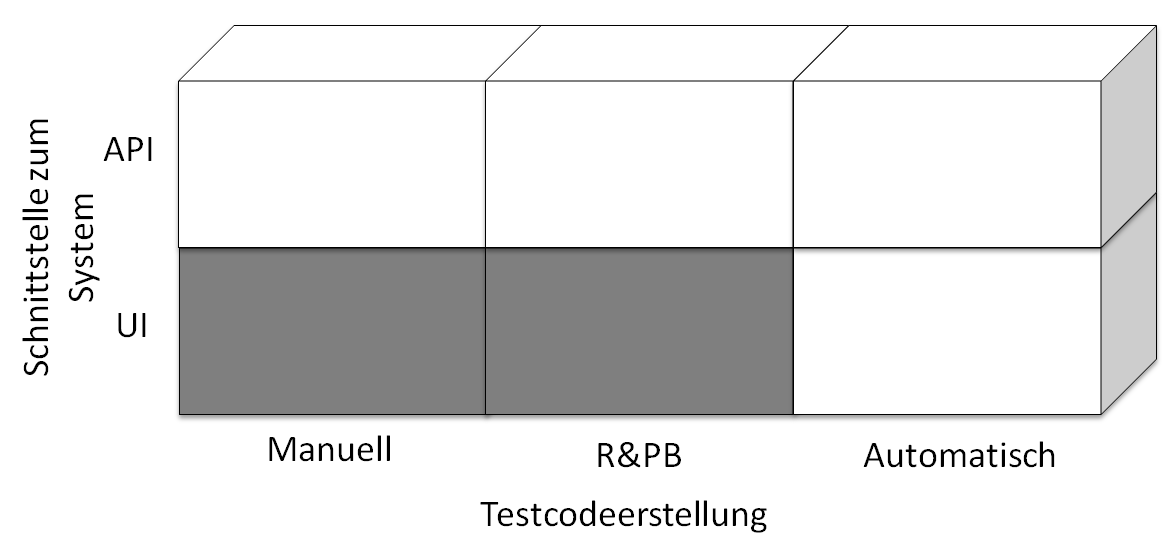
\includegraphics[scale=0.7]{img/bereicheTestcodeerstellungSelenium.png}\\
  \footnotesize\sffamily\textbf{Quelle:} vgl. \cite{meszaros_agile_2003}
  \caption{Einordnung von Selenium in die verschiedene Möglichkeiten der Testcodeerstellung}
  \label{fig:bereicheTestcodeerstellungSelenium}
\end{figure}
Genau genommen handelt es sich bei Selenium aber nicht um ein einzelnes Tool, sondern um eine Reihe von Tools die unter dem Namen Selenium zusammengefasst werden.
In seiner aktuellen Ausprägung 2.x lassen sich, abgesehen von Komponenten die der Abwärtskompatibilität dienen, laut Dokumentation \cite{selenium_selenium_2015-1} drei Komponenten unterscheiden:

\begin{itemize}
\item Selenium IDE \\
Bei der Selenium IDE handelt es sich um ein Firefox plug-in, das verwendet werden kann um Selenium-Testfälle zu erstellen. Testfälle können dabei von Hand erstellt werden oder mittels eines \grq record-and playback\grq -Mechanismus direkt im Browser aufgezeichnet werden. Die erstellten Testfälle können mit Akzeptanzkriterien angereichert werden und innerhalb der IDE wieder abgespielt werden.
\item Selenium WebDriver \\
Der Selenium WebDriver bietet für verschiedene Programmiersprachen eine API zur Steuerung eines Browsers aus dem Programmcode heraus. Der WebDriver bildet damit die Kernkomponente für alle Selenium-Testfälle die außerhalb der Selenium IDE entwickelt werden.

\item Selenium Server/Grid \\
Mit Hilfe des Selenium Servers ist es möglich Selenium-Testfälle nicht nur auf dem eigenen Rechner auszuführen sondern die Ausführung auf einen Server auszulagern. Einen wichtigen Teil des Selenium Server bildet Selenium Grid. Selenium Grid bietet die Möglichkeit die Ausführung von Selenium-Testfällen über einen Server hinaus auf eine Vielzahl von Knoten zu verteilen. Selenium Server dient dann als Hub der die Testfallanfragen auf Registriert Knoten zur Ausführung weiterleitet. 
\end{itemize}


\section{Testdurchführung mit Selenium}
\label{sec:testdurchführung_mit_selenium}
Abhängig davon ob die Testfälle für die Selenium IDE entwickelt wurden oder sich auf den Selenium WebDriver stützen unterscheiden sich die Möglichkeiten zur Ausführung der Testskripte.\\
Testfälle die mit der Selenium IDE entwickelt wurden verwenden eine Selenium eigene Sprache mit dem Namen \grq Selense\grq.\ Diese Testfälle können in späteren Testläufen wieder über die Selenium IDE zur Ausführung gebracht werden. \\
Testfälle die mittels Selenium WebDriver entwickelt wurden sind für ihre Ausführung nicht an ein spezielles Tool gebunden. Beim WebDriver handelt es sich um eine API mit deren Hilfe ein Browser ferngesteuert werden kann. Wie diese API in die Testfälle integriert wird ist dem Entwickler selbst überlassen. In der Praxis hat sich als Best Practice jedoch herausgestellt, dass Selenium-Testfälle, die den WebDriver verwenden, meist in Verbindung mit einem Unit Testing Framework entwickelt werden.
Im Java Umfeld wären hier beispielsweise JUnit oder TestNG zu nennen.
Die Testfälle können damit analog zu den klassischen Unit Tests entwickelt werden, verwenden jedoch als Schnittstelle zum System nicht die API sondern, über den WebDriver, die Benutzeroberfläche. 
Die Ausführung der Testfälle erfolgt dann analog zu den klassischen Unit Tests über das Unit Testing Framework.
Im Bereich des WebDrivers stützt sich Selenium also auf bereits sehr gut etablierte Frameworks. Das hat den Vorteil, dass die so erstellten Testfälle bereits in den meisten Programmiersprachen gut in die Infrastruktur integriert sind. In Java sind Testfälle die mittels JUnit ausgeführt werden in allen gängigen IDEs durch Plugins unterstützt. Noch viel wichtiger ist jedoch eine gute Integration der Testfälle in den Buildprozess. Werden beispielsweise in Java Standarttools wie Gradle oder Maven zum bauen der Projekte verwendet, können die Testfälle ohne Mehraufwand im Rahmen des Buildprozesses ausgeführt werden.



\section{Testcodeerstellung mit Selenium}
\label{sec:Testdesign}


\subsection{Recorde-and-playback}
\label{sec:recorde_and_playback}


\subsubsection{Vorteile von Recorde-and-playback}
\label{sec:vorteile_von_recorde_and_playback}

\subsubsection{Probleme von Recorde-and-playback}
\label{sec:probleme_von_recorde_and_playback}

\subsection{Manuell}
\label{sec:manuell}

\subsection{Page Object Pattern}
\label{sec:page_object_pattern}

\subsubsection{Vorteile des Page Object Pattern}
\label{sec:vorteile_des_page_object_pattern}

\subsubsection{Probleme des Page Object Pattern}
\label{sec:probleme_des_page_object_pattern}



